\documentclass{standalone}
\usepackage{pgfplots}
\pgfplotsset{compat=1.18}

\begin{document}

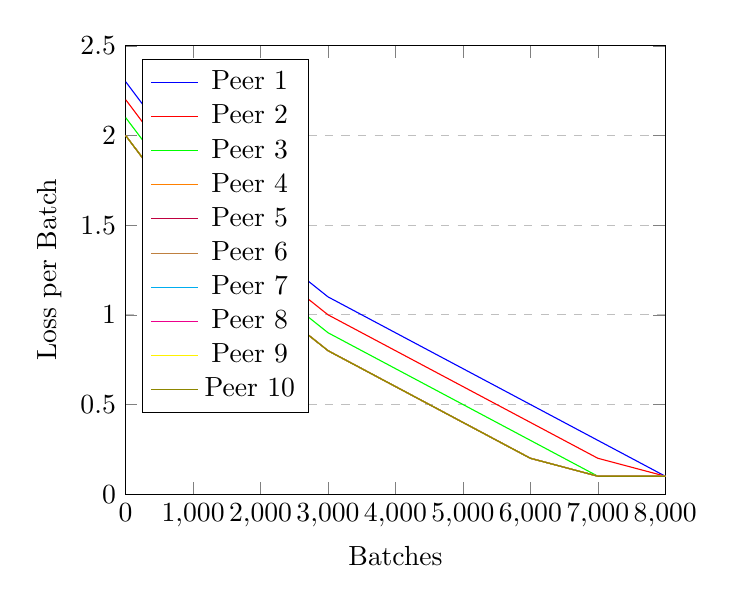
\begin{tikzpicture}
    \begin{axis}[
        xlabel={Batches},
        ylabel={Loss per Batch},
        xmin=0, xmax=8000,
        ymin=0, ymax=2.5,
        xtick={0,1000,...,8000},
        ytick={0,0.5,1,1.5,2,2.5},
        legend pos=north west,
        ymajorgrids=true,
        grid style=dashed,
    ]
    
    % Example data for each peer
    \addplot[blue] coordinates {
        (0, 2.3)
        (1000, 1.8)
        (2000, 1.4)
        (3000, 1.1)
        (4000, 0.9)
        (5000, 0.7)
        (6000, 0.5)
        (7000, 0.3)
        (8000, 0.1)
    };
    \addlegendentry{Peer 1};
    
    \addplot[red] coordinates {
        (0, 2.2)
        (1000, 1.7)
        (2000, 1.3)
        (3000, 1.0)
        (4000, 0.8)
        (5000, 0.6)
        (6000, 0.4)
        (7000, 0.2)
        (8000, 0.1)
    };
    \addlegendentry{Peer 2};
    
    \addplot[green] coordinates {
        (0, 2.1)
        (1000, 1.6)
        (2000, 1.2)
        (3000, 0.9)
        (4000, 0.7)
        (5000, 0.5)
        (6000, 0.3)
        (7000, 0.1)
        (8000, 0.1)
    };
    \addlegendentry{Peer 3};
    
    \addplot[orange] coordinates {
        (0, 2.0)
        (1000, 1.5)
        (2000, 1.1)
        (3000, 0.8)
        (4000, 0.6)
        (5000, 0.4)
        (6000, 0.2)
        (7000, 0.1)
        (8000, 0.1)
    };
    \addlegendentry{Peer 4};
    
    \addplot[purple] coordinates {
        (0, 2.0)
        (1000, 1.5)
        (2000, 1.1)
        (3000, 0.8)
        (4000, 0.6)
        (5000, 0.4)
        (6000, 0.2)
        (7000, 0.1)
        (8000, 0.1)
    };
    \addlegendentry{Peer 5};
    
    \addplot[brown] coordinates {
        (0, 2.0)
        (1000, 1.5)
        (2000, 1.1)
        (3000, 0.8)
        (4000, 0.6)
        (5000, 0.4)
        (6000, 0.2)
        (7000, 0.1)
        (8000, 0.1)
    };
    \addlegendentry{Peer 6};
    
    \addplot[cyan] coordinates {
        (0, 2.0)
        (1000, 1.5)
        (2000, 1.1)
        (3000, 0.8)
        (4000, 0.6)
        (5000, 0.4)
        (6000, 0.2)
        (7000, 0.1)
        (8000, 0.1)
    };
    \addlegendentry{Peer 7};
    
    \addplot[magenta] coordinates {
        (0, 2.0)
        (1000, 1.5)
        (2000, 1.1)
        (3000, 0.8)
        (4000, 0.6)
        (5000, 0.4)
        (6000, 0.2)
        (7000, 0.1)
        (8000, 0.1)
    };
    \addlegendentry{Peer 8};
    
    \addplot[yellow] coordinates {
        (0, 2.0)
        (1000, 1.5)
        (2000, 1.1)
        (3000, 0.8)
        (4000, 0.6)
        (5000, 0.4)
        (6000, 0.2)
        (7000, 0.1)
        (8000, 0.1)
    };
    \addlegendentry{Peer 9};
    
    \addplot[olive] coordinates {
        (0, 2.0)
        (1000, 1.5)
        (2000, 1.1)
        (3000, 0.8)
        (4000, 0.6)
        (5000, 0.4)
        (6000, 0.2)
        (7000, 0.1)
        (8000, 0.1)
    };
    \addlegendentry{Peer 10};
    
    \end{axis}
\end{tikzpicture}

\caption{Rolling mean (with window = 500) of loss per batch for 10 peers within the same shard. Each color represents the loss of one of the peers.}
\label{fig:rolling_mean_loss}

\end{document}